\documentclass[12pt,english]{article}
\usepackage[a4paper,top=5mm, bottom=15mm]{geometry}
\usepackage{graphicx}
\usepackage{amssymb}
\usepackage{amsmath}
\usepackage[numbers]{natbib}
\usepackage{booktabs}
\usepackage{subcaption}
\usepackage[capitalise]{cleveref}

\usepackage{graphicx}
\graphicspath{{./figures/}}
\DeclareGraphicsExtensions{.pdf,.jpeg,.png,.jpg}

\newcommand{\ie}{i.e.,}
\newcommand{\eg}{e.g.,}
\newcommand*{\hurl}[1]{\href{http://#1}{\emph{#1}}}
\let\biconditional\leftrightarrow%

\pagestyle{empty}

\title{Using the Multi-Agent Deep Deterministic Policy Gradient Algorithm to Solve the Tennis Environment}
\author{Alessandro Leite}

\date{}

\pagenumbering{gobble}

\begin{document}
\maketitle
\thispagestyle{plain}
\vspace{-60pt}

\section{Context}\label{sec:introduction}

An important concept in machine learning comprises the tasks of deciding from experience the sequence of action to perform in an uncertain environment to achieve some objective~\cite{francois:18}. Inspired by behavioral psychology~\cite{sutton:18}, reinforcement learning~(RL) proposes a formal framework in which an agent learns by iterating with an environment. Based on experiences gathered by this iteration, the agent learns to optimize some objectives represented in the form of cumulative rewards. Thus, reinforcement learning focuses on the problem of learning a behavioral policy, a mapping from states to actions, which maximizes cumulative long-term rewards~\cite{sutton:18}. A policy can be represented as a lookup table, listing the appropriate action from any state. Therefore, in a rich environment, this approach is infeasible, and the policy must be encoded as a parametrized function.

Over the last years, RL has achieved some breakthroughs by integrating deep learning techniques. This combination, named deep reinforcement learning~(DRL) is appropriate for problems with high dimensional spaces. As a result, deep reinforcement learning can learn different levels of abstractions from the data, which helps it to be successfully employed in complicated tasks with lower prior knowledge.   

\section{Goal}

This project uses the Unity platform to train two agents to play tennis. In this case, two agents control rackets to bounce a ball over a net. If an agent hits the ball over the net, it receives a reward of \(+0.1\). If an agent lets a ball hit the ground or hits the ball out of bounds, it receives a reward of \(-0.01\).  Thus, the goal of each agent is to keep the ball in play.

The observation space consists of eight variables corresponding to the position and velocity of the ball and racket. Each agent receives its own, local observation. Two continuous actions are available, corresponding to movement toward or away from the net, and jumping. The task is episodic, and in order to solve the environment, the agents must get an average score of \(+0.5\) over \(100\) consecutive episodes to considered the environment as solved. 

\section{Method}

The proposed solution relies on Deep Deterministic Policy Gradient~(DDPG) algorithm proposed by~\citeauthor{lillicrap:16}~\cite{lillicrap:16}. DDPG is an off-policy actor-critic algorithm that uses deep function approximators to learn policies in high-dimensional continuous action spaces. It is based on the deterministic policy gradient algorithm~(DGP) algorithm~\citeauthor{silver:14}. DPG algorithm maintains an actor function \(\mu(s|\theta^\mu)\) to specify an policy that maps states to a specific action. Similar to Q-learning, the critic \(Q(s,a)\) function relies on Bellman equation and the actor is updated by applying the chain rule to the expected return from the start distribution \(J\) with respect to the actor parameters~\cite{lillicrap:16}:

\begin{equation*}
   \begin{aligned}
      \nabla_{\theta^{\mu}} J & \approx \mathbb{E}_{s_{t} \sim \rho^{\beta}}\left[\left.\nabla_{\theta^{\mu}} Q\left(s, a | \theta^{Q}\right)\right|_{s=s_{t}, a=\mu\left(s_{t} | \theta^{\mu}\right)}\right] \\&=\mathbb{E}_{s_{t} \sim \rho^{\beta}}\left[\left.\left.\nabla_{a} Q\left(s, a | \theta^{Q}\right)\right|_{s=s_{t}, a=\mu\left(s_{t}\right)} \nabla_{\theta_{\mu}} \mu\left(s | \theta^{\mu}\right)\right|_{s=s_{t}}\right]
   \end{aligned}
\end{equation*}

Exploration is one major challenge of learning in continuous action spaces. Therefore, off-policy algorithms such as DDPG can handle the exploration problem independent from the learning algorithm. The DDPG algorithm employs an exploration policy \(\mu^\prime\) by adding noise sampled from an Ornstein-Uhlenbeck process~\(\mathcal{N}\) to the actor policy. 

\begin{equation*}
\mu^{\prime}\left(s_{t}\right)=\mu\left(s_{t} | \theta_{t}^{\mu}\right)+\mathcal{N}
\end{equation*}

\section{Results}

The architecture is the same one proposed by \citeauthor{lillicrap:16}\cite{lillicrap:16}. Different from the original implementation, this work updates the actor and critic network \(10\) times every \(20\) steps. \Cref{tb:parameters} illustrates the values of the parameters of the networks. 

\Cref{fig:score} shows the performance of DDPG algorithm when solving the Reacher task. The algorithm required \(360\) episodes to solve the task.

For this kind of environment, the algorithms that employ a distributed approach to distribute the tasks usually lead to a better performance.

\begin{table}
\footnotesize
{
  \caption{Hyperparameters}\label{tb:parameters}
  \centering
  \begin{tabular}{cccccc}
  \toprule
    \textbf{buffer size} & \textbf{mini-batch} & \textbf{discount factor} & \textbf{LR actor} & \textbf{LR critic} & \textbf{soft updates}\\
  \midrule
   \(10^6\) & 200 & \(\gamma = 0.99\) & \(\alpha_{\text{actor}} = 10^{-4}\) & \(\alpha_{\text{critic}} = 10^{-3}\) & \(\tau=10^{-3}\)\\
  \bottomrule
  \end{tabular}
}
\end{table}

\begin{figure*}%[t!]
    \centering
    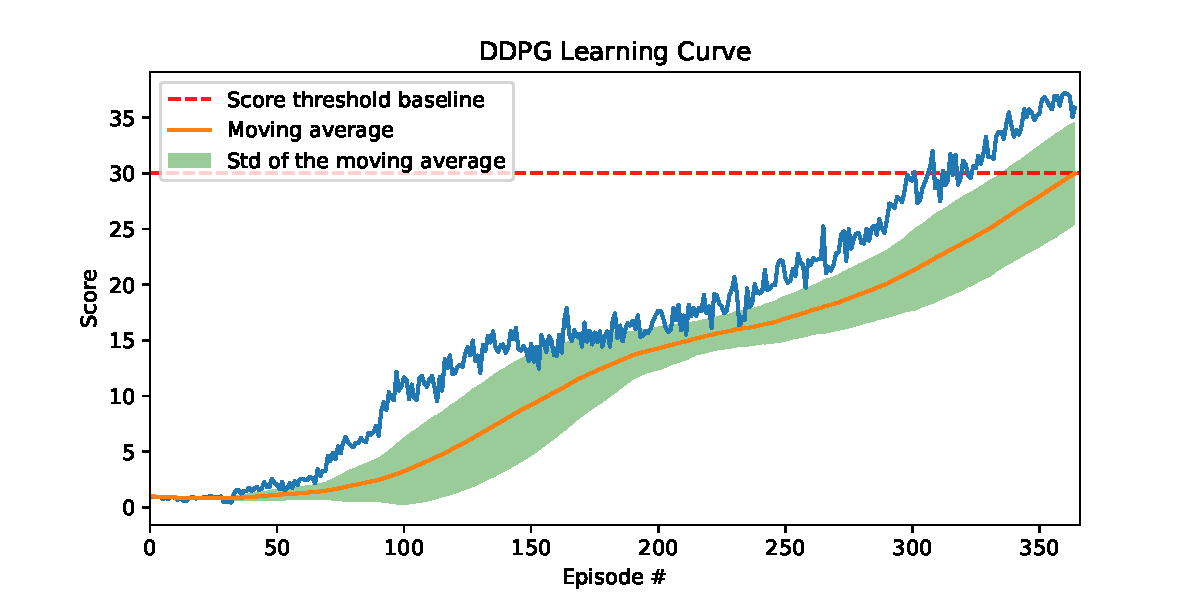
\includegraphics[width=\textwidth]{ddpg_score}
    \caption{Learning curve of the DDPG algorithms}\label{fig:score}
\end{figure*}

\bibliographystyle{IEEEtranN}
\bibliography{references}
\end{document}  